\documentclass[11pt, a4paper]{article}
\usepackage[margin=1.8cm]{geometry} % permet de faire les marges personnalisées 
\usepackage{graphicx} % permet d'insérer des photos 
\usepackage{hyperref} % permet de faire des liens cliquables 

\usepackage{tabularx} % permet d'effectuer les aspects avec les dates puis les formations etc... 

\hypersetup{
    colorlinks=true,
    urlcolor=black,
    linkcolor=black
}


\pagestyle{empty} % supprime les numéros en bas de page

\begin{document}

% Bloc titre à centrer 
\noindent
\begin{minipage}[c]{1cm}
    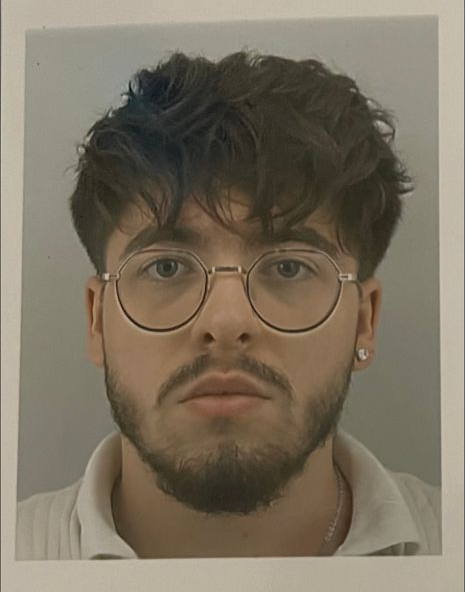
\includegraphics[width=2.5cm]{photo_identite_Lorenzo.png}
\end{minipage}
\hfill
\begin{minipage}[c]{0.75\textwidth}
\centering
{\LARGE \textbf{DERREZ Lorenzo}}\\
+33 7 50 69 25 61 \quad | \quad \href{mailto:lrdrz.professionnel@gmail.com}{lrdrz.professionnel@gmail.com} \quad | \quad \href{https://www.linkedin.com/in/lorenzo-derrez}{LinkedIn} \quad | \quad \href{https://github.com/Nmrodd}{GitHub}
\end{minipage}
\hfill
\begin{minipage}[c]{1cm}
\end{minipage}

\begin{flushleft} % permet d'insérer du text à gauche 
    \large \textit{Elève-ingénieur en Informatique - ENSEIRB-MATMECA Bordeaux}
    \\
    \small Curieux, Co-worker, Rigoureux, Discipliné, Perfectionniste
\end{flushleft}

\rule{\textwidth}{0.4pt}  % permet de tracer le trait 

\section*{Formation} % * permet d'enlever le comportement automatique de numérotation 

\begin{tabularx}{\textwidth}{@{}l X r@{}}
    2021 --  2024 & \textbf{Lycée Beau-Jardin / Baccalauréat} \quad \textit{Saint-Dié-des-Vosges}
    \\
    & \small Mention Très Bien -- Spécialités Mathématiques, NSI, Physique-Chimie & \\[4pt]
    2024 -- 2026 & \textbf{Classes préparatoires aux grandes écoles / Lycée Henri-Poincaré} \quad \textit{Nancy}
    \\
    2026 -- 2029 & \textbf{École d’ingénieur ENSEIRB-MATMECA} \quad \textit{Bordeaux}
\end{tabularx}

\vspace{2pt}
\rule{\textwidth}{0.4pt}  % permet de tracer le trait 

\section*{Expériences}

\subsection*{Compétences}

\begin{tabularx}{\textwidth}{@{}l X r@{}}
    -- 3 ans : & \textbf{Langage C}
    \\
    -- 3 ans : & \textbf{Python}
    \\
    -- 2 ans : & \textbf{Langage OCamL} 
    \\
    -- 1 an : & \textbf{LaTex, VIM}
    \\
    -- & \textbf{Français}
    \\
    --  \textbf{C2} : & \textbf{Anglais}
    \\
    -- \textbf{B2} : & \textbf{Italien}
\end{tabularx}

\vspace{2pt}
\rule{\textwidth}{0.4pt}  % permet de tracer le trait 

\subsection*{Stages}

\begin{tabularx}{\textwidth}{@{}l X r@{}}
    2022 & \textbf{Numalliance} \quad \textit{Fabricant de machines automatisées}
    \\
    2024 & \textbf{EY Luxembourg} \quad \textit{Pôle Cybersécurité}
\end{tabularx}

\vspace{2pt}
\rule{\textwidth}{0.4pt}  % permet de tracer le trait 

\subsection*{Séjours linguistiques}

\begin{tabularx}{\textwidth}{@{}l X r@{}}
    2019 & \textbf{Londres} \quad \textit{Classe européenne}
    \\
    2023 & \textbf{San Francisco} \quad \textit{Année de terminale, cursus de LV1}
    \\
    2023 & \textbf{Italie} \quad \textit{Cursus de LV2}
\end{tabularx}

\vspace{2pt}
\rule{\textwidth}{0.4pt}  % permet de tracer le trait 

\subsection*{Associatif}

\begin{tabularx}{\textwidth}{@{}l X r@{}}
    -- Participation à des journées de nettoyage et de dépollution des villes 
    \\
    -- Organisation de la commémoration du 11 novembre
    \\
    -- Participation à des travaux de chantiers jeunes dans les communes 
    \\
    -- Participation à des associations étudiantes au sein de mes divers établissements 

\end{tabularx}

\vspace{2pt}
\rule{\textwidth}{0.4pt}  % permet de tracer le trait 

\subsection*{Sport}

\begin{tabularx}{\textwidth}{@{}l X r@{}}
    -- \textbf{Basket-ball} \quad \textit{Club et associatif durant une décennie}
    \\
    -- \textbf{Musculation} \quad \textit{En autodidacte}
    \\
    -- \textbf{Boxe} \quad \textit{En autodidacte}
\end{tabularx}

\end{document}